\documentclass{article}
\usepackage{graphicx} % Required for inserting images
\usepackage{amsmath}
\usepackage[a4paper,top=1.8cm,bottom=1.8cm,left=2cm,right=2cm]{geometry}
\usepackage{amssymb}
\usepackage{enumitem} % Options de mise en forme des listes enumerate
\usepackage{tikz} % Requis pour les graphes des questions 5 et 6
\usepackage{float}

% Commande personnalisée pour le symbole d'indépendance
\newcommand{\indep}{\perp \!\!\! \perp}

% Mise en forme des conclusions, avec retour à la ligne dans les encadrés
\newcommand{\conclusion}[1]{%
  \begin{center}
    \setlength{\fboxsep}{6pt}%
    \fbox{\parbox{0.9\linewidth}{\centering #1}}%
  \end{center}}

\title{STT760 - Devoir 1}
\author{Équipe 1 :\\
    AMOUDRUZ Louis (amol5580) \\
    BASTARDIE Dimitri (basd5079) \\
    CAMPILLO-LAFFIN Corentin (camc1598) \\
    MITURA Corentin (mitc2657) \\
    PONSSARD Jules (ponj3185) 
}
\date{09/10/2026}

\begin{document}

\maketitle

\section*{Question 1}

On considère trois variables aléatoires binaires
\[
X_1,X_2,X_3\in\{0,1\},
\]
telles que
\[
X_1 \perp\!\!\!\perp X_2,
\qquad
P(X_1=1)=P(X_2=1)=\frac12,
\]
et
\[
X_3
=
I(X_1=1,X_2=0)
+
I(X_1=0,X_2=1).
\]

\subsection*{a) Calcul de $P(X_3=1)$ et $P(X_3=0)$}

Posons
\[
A=\{X_1=1,X_2=0\},
\qquad
B=\{X_1=0,X_2=1\}.
\]

On a $X_3=1 \iff A\cup B$. Les événements $A$ et $B$ sont disjoints et, comme
$X_1$ et $X_2$ sont indépendantes,
\[
P(A)=P(X_1=1)P(X_2=0)=\frac12\cdot\frac12=\frac14,
\qquad
P(B)=\frac14.
\]
et de même
\[
P(B)=\frac14.
\]

Ainsi,
\[
P(X_3=1)
=
P(A)+P(B)
=
\frac14+\frac14
=
\frac12.
\]

Par conséquent,
\[
P(X_3=0)
=
1-P(X_3=1)
=
\frac12.
\]

Donc
\[
P(X_3=1)=P(X_3=0)=\frac12.
\]

\subsection*{b) Montrer que $X_3 \perp\!\!\!\perp X_1$ et $X_3 \perp\!\!\!\perp X_2$}

Si $X_1=1$, alors
\[
X_3=1
\iff X_2=0.
\]

Par conséquent,
\[
P(X_3=1\mid X_1=1)
=
P(X_2=0\mid X_1=1).
\]

Comme $X_1$ et $X_2$ sont indépendantes,
\[
P(X_2=0\mid X_1=1)
=
P(X_2=0)
=
\frac12.
\]

Or,
\[
P(X_3=1)=\frac12.
\]

Ainsi,
\[
P(X_3=1\mid X_1=1)
=
P(X_3=1).
\]

De même, si $X_1=0$, alors
\[
X_3=1
\iff X_2=1,
\]
et donc
\[
P(X_3=1\mid X_1=0)
=
P(X_2=1)
=
\frac12
=
P(X_3=1).
\]

On en déduit que
\[
X_3 \perp\!\!\!\perp X_1.
\]

Par symétrie, on obtient également
\[
X_3 \perp\!\!\!\perp X_2.
\]

\subsection*{c) Montrer que $X_3 \not\!\perp\!\!\!\perp (X_1,X_2)$}

Considérons le cas
\[
X_1=1,
\qquad
X_2=0.
\]

Par définition de $X_3$, on a alors nécessairement
\[
X_3=1.
\]

Ainsi,
\[
P(X_3=1\mid X_1=1,X_2=0)=1.
\]

Or,
\[
P(X_3=1)=\frac12.
\]

Donc
\[
P(X_3=1\mid X_1=1,X_2=0)
\neq
P(X_3=1),
\]
ce qui montre que
\[
X_3 \not\!\perp\!\!\!\perp (X_1,X_2).
\]

\subsection*{d) Bonus : existence d'une SRB carte parfaite de $P$}

On a montré que
\[
X_1 \perp\!\!\!\perp X_2,
\qquad
X_1 \perp\!\!\!\perp X_3,
\qquad
X_2 \perp\!\!\!\perp X_3.
\]

Les trois variables sont donc indépendantes deux à deux.

Cependant,
\[
X_3 \not\!\perp\!\!\!\perp (X_1,X_2).
\]

Une SRB sans aucune arête représenterait une indépendance mutuelle complète, notamment
\[
X_1 \perp\!\!\!\perp (X_2,X_3),
\]
ce qui est faux.

À l'inverse, si l'on ajoute une arête entre deux variables, celles-ci ne sont plus d-séparées marginalement, alors qu'elles doivent être indépendantes.

Ainsi, aucune SRB ne peut représenter exactement toutes les indépendances de $P$.

Donc,
\[
\text{il n'existe pas de SRB qui soit une carte parfaite des indépendances de }P.
\]

\vspace{1cm}
\hrule
\vspace{1cm}

\section*{Question 2}

On considère $x_1,\ldots,x_n$ des réalisations indépendantes d'une variable aléatoire
\[
X \sim \operatorname{Poisson}(\lambda),
\]
dont la fonction de masse est
\[
p_\lambda(x)
=
\frac{\lambda^x e^{-\lambda}}{x!},
\qquad x\in\mathbb{N}.
\]

\textbf{a) Estimateur du maximum de vraisemblance}

Comme les observations sont indépendantes, la vraisemblance s'écrit
\[
L(\lambda)
=
\prod_{i=1}^n p_\lambda(x_i)
=
\prod_{i=1}^n
\frac{\lambda^{x_i}e^{-\lambda}}{x_i!}.
\]

On peut regrouper les termes :
\[
L(\lambda)
=
\frac{
\lambda^{\sum_{i=1}^n x_i}
e^{-n\lambda}
}{
\prod_{i=1}^n x_i!
}.
\]

On considère la log-vraisemblance
\[
\ell(\lambda)=\log L(\lambda),
\]
qui admet les mêmes maximiseurs que $L(\lambda)$ puisque le logarithme est strictement croissant.

Ainsi,
\[
\ell(\lambda)
=
\left(\sum_{i=1}^n x_i\right)\log(\lambda)
-
n\lambda
-
\sum_{i=1}^n \log(x_i!).
\]

En posant
\[
\bar{x}
=
\frac{1}{n}\sum_{i=1}^n x_i,
\]
on a
\[
\sum_{i=1}^n x_i=n\bar{x}.
\]

Donc
\[
\ell(\lambda)
=
n\bar{x}\log(\lambda)
-
n\lambda
-
\sum_{i=1}^n \log(x_i!).
\]

On dérive par rapport à $\lambda$ :
\[
\ell'(\lambda)
=
\frac{n\bar{x}}{\lambda}
-
n.
\]

On cherche le point critique en posant
\[
\ell'(\lambda)=0.
\]

On obtient
\[
\frac{n\bar{x}}{\lambda}-n=0,
\]
donc
\[
\frac{\bar{x}}{\lambda}=1.
\]

Ainsi,
\[
\hat{\lambda}=\bar{x}.
\]

Pour vérifier qu'il s'agit bien d'un maximum, on calcule la dérivée seconde :
\[
\ell''(\lambda)
=
-\frac{n\bar{x}}{\lambda^2}.
\]

Comme au moins une des observations est non nulle, on a $\bar{x}>0$, donc
\[
\ell''(\lambda)<0.
\]

La log-vraisemblance est donc concave et le point critique correspond bien à un maximum.

Ainsi,
\[
\hat{\lambda}
=
\bar{x}
=
\frac{1}{n}\sum_{i=1}^n x_i.
\]

\bigskip

\textbf{b) Valeur numérique de l'estimateur}

Pour l'échantillon
\[
3,\ 2,\ 4,\ 0,\ 1,\ 3,\ 2,\ 5,\ 2,\ 1,
\]
on a
\[
\bar{x}
=
\frac{3+2+4+0+1+3+2+5+2+1}{10}.
\]

Donc
\[
\bar{x}
=
\frac{23}{10}
=
2.3.
\]

Finalement,
\[
\hat{\lambda}
=
\bar{x}
=
2.3.
\]
\vspace{1cm}
\hrule
\vspace{1cm}

\section*{Question 3}

\subsection*{a) Réseau $G_1$}

On considère la SRB
\[
X_1 \longrightarrow X_2 \longrightarrow X_3.
\]

\subsubsection*{(i) Ensemble des indépendances globales $I(G_1)$}

Dans le graphe
\[
X_1 \longrightarrow X_2 \longrightarrow X_3,
\]
le seul chemin entre $X_1$ et $X_3$ passe par $X_2$.

Le conditionnement sur $X_2$ bloque donc ce chemin.

Ainsi,
\[
I(G_1)
=
\left\{
X_1 \perp\!\!\!\perp X_3 \mid X_2
\right\}.
\]

\subsubsection*{(ii) SRB I-équivalentes à $G_1$}

Deux SRB sont I-équivalentes si elles ont le même squelette et les mêmes v-structures.

Le squelette de $G_1$ est
\[
X_1-X_2-X_3.
\]

Le graphe $G_1$ ne contient aucune v-structure.

Les orientations possibles conservant le même squelette sans créer de v-structure sont donc
\[
X_1 \longrightarrow X_2 \longrightarrow X_3,
\]

\[
X_1 \longleftarrow X_2 \longrightarrow X_3,
\]

et
\[
X_1 \longleftarrow X_2 \longleftarrow X_3.
\]

Le graphe
\[
X_1 \longrightarrow X_2 \longleftarrow X_3
\]
n'est pas I-équivalent à $G_1$, car il contient une v-structure en $X_2$.

Ainsi, il y a exactement trois SRB I-équivalentes à $G_1$, en comptant $G_1$ lui-même.

\subsubsection*{(iii) $G_1$ est-il une carte parfaite des indépendances de $P$ ?}

La distribution est donnée par
\[
P(X_1,X_2,X_3)
=
0.2^{X_1+X_3}
0.8^{2-X_1-X_3}
\left(
\frac{X_3+0.5}{2}
\right)^{X_2}
\left(
1-\frac{X_3+0.5}{2}
\right)^{1-X_2}.
\]

On peut réécrire
\[
0.2^{X_1+X_3}
0.8^{2-X_1-X_3}
\]
sous la forme
\[
\left(
0.2^{X_1}0.8^{1-X_1}
\right)
\left(
0.2^{X_3}0.8^{1-X_3}
\right).
\]

Ainsi,
\[
P(X_1,X_2,X_3)
=
\left(
0.2^{X_1}0.8^{1-X_1}
\right)
\left[
0.2^{X_3}0.8^{1-X_3}
\left(
\frac{X_3+0.5}{2}
\right)^{X_2}
\left(
1-\frac{X_3+0.5}{2}
\right)^{1-X_2}
\right].
\]

On peut donc écrire
\[
P(X_1,X_2,X_3)
=
f(X_1)g(X_2,X_3).
\]

Cette factorisation implique que
\[
X_1 \perp\!\!\!\perp (X_2,X_3).
\]

En particulier,
\[
X_1 \perp\!\!\!\perp X_2
\]
et
\[
X_1 \perp\!\!\!\perp X_3.
\]

Or ces indépendances marginales ne sont pas représentées par $G_1$. En effet, dans
\[
X_1 \longrightarrow X_2 \longrightarrow X_3,
\]
$X_1$ et $X_2$ ne sont pas d-séparées.

Ainsi,
\[
I(G_1)\neq I(P).
\]

Par conséquent,
\[
G_1
\text{ n'est pas une carte parfaite des indépendances de }P.
\]

\vspace{1cm}
\hrule
\vspace{1cm}

\section*{Question 4}
\begin{center}
  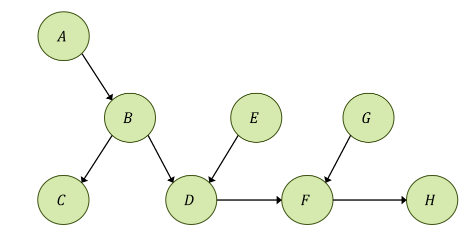
\includegraphics[width=0.9\textwidth]{q4.png}
\end{center}

\section*{a) Assertions d'indépendance}

\begin{enumerate}[label=(\roman*), leftmargin=*, itemsep=1.5em]

% ---------------------------------------------------------------- (i)
\item On considère le parcours $A \to B \to D \to F \leftarrow G$.
Ce parcours est actif étant donné $H$ car :
\begin{itemize}
  \item $A \to B \to D$ et $B \notin \{H\}$
  \item $B \to D \to F$ et $D \notin \{H\}$
  \item $D \to F \leftarrow G$ et $H$ est un descendant de $F$
\end{itemize}
Donc $(A,C)$ et $G$ ne sont pas d-séparés étant donné $H$, car il existe un parcours actif entre $A \in (A,C)$ et $G$ étant donné $H$.
\conclusion{Ainsi $(A,C) \indep G \mid H$ est \textbf{faux}.}

% --------------------------------------------------------------- (ii)
\item Le seul parcours reliant $E$ et $G$ est $E \to D \to F \leftarrow G$, qui passe par la v-structure $D \to F \leftarrow G$.
Or le n\oe ud $F$ et son descendant $H$ n'appartiennent pas à $\emptyset$.
Donc il n'existe pas de parcours actif entre $E$ et $G$ étant donné $\emptyset$ : ils sont d-séparés étant donné $\emptyset$.
\conclusion{Ainsi $E \indep G \mid \emptyset$ est \textbf{vrai}.}

% -------------------------------------------------------------- (iii)
\item On considère le parcours $A \to B \to D \leftarrow E$.
Ce parcours est actif étant donné $H$ car :
\begin{itemize}
  \item $A \to B \to D$ et $B \notin \{H\}$
  \item $B \to D \leftarrow E$ et $H$ est un descendant de $D$
\end{itemize}
Donc $A$ et $E$ ne sont pas d-séparés étant donné $H$, car il existe un parcours actif entre $A$ et $E$ étant donné $H$.
\conclusion{Ainsi $A \indep E \mid H$ est \textbf{faux}.}

% --------------------------------------------------------------- (iv)
\item On considère le parcours $A \to B \to D \leftarrow E$.
Ce parcours est actif étant donné $D$ car :
\begin{itemize}
  \item $A \to B \to D$ et $B \notin \{D\}$
  \item $B \to D \leftarrow E$ et $D \in \{D\}$
\end{itemize}
Donc $A$ et $(E,C)$ ne sont pas d-séparés étant donné $D$, car il existe un parcours actif entre $A$ et $E \in (E,C)$ étant donné $D$.
\conclusion{Ainsi $A \indep (E,C) \mid D$ est \textbf{faux}.}

% ---------------------------------------------------------------- (v)
\item Le seul parcours reliant $C$ et $E$ est $C \leftarrow B \to D \leftarrow E$, qui passe par la v-structure $B \to D \leftarrow E$.
Or le n\oe ud $D$ et tous ses descendants ($F$ et $H$) n'appartiennent pas à $\{A\}$.
Donc il n'existe pas de parcours actif entre $C$ et $E$ étant donné $A$ : $C$ et $E$ sont d-séparés étant donné $A$.
\conclusion{Ainsi $C \indep E \mid A$ est \textbf{vrai}.}

% --------------------------------------------------------------- (vi)
\item On considère le parcours $A \to B \to D \to F$.
Ce parcours est actif étant donné $\emptyset$ car :
\begin{itemize}
  \item $A \to B \to D$ et $B \notin \emptyset$
  \item $B \to D \to F$ et $D \notin \emptyset$
\end{itemize}
Donc $A$ et $F$ ne sont pas d-séparés étant donné $\emptyset$, car il existe un parcours actif entre $A$ et $F$ étant donné $\emptyset$.
\conclusion{Ainsi $A \indep F \mid \emptyset$ est \textbf{faux}.}

% -------------------------------------------------------------- (vii)
\item Tous les parcours reliant $C$ et $G$ passent par la structure $C \leftarrow B \to D$ et $B \in \{F,B\}$.
Donc il n'existe pas de parcours actif reliant $C$ et $G$ étant donné $\{F,B\}$ : $C$ et $G$ sont d-séparés étant donné $\{F,B\}$.
\conclusion{Ainsi $C \indep G \mid (F,B)$ est \textbf{vrai}.}

\end{enumerate}

\section*{b) SRB I-équivalentes}
 
L'affirmation est fausse car on trouve deux SRB I-équivalentes à celle donnée en a) et différentes de celle-ci.
On conserve les arêtes $B \to D \leftarrow E$, $D \to F \leftarrow G$ et $F \to H$ et on modifie seulement l'orientation de $A - B - C$ sans créer de nouvelle v-structure :
\begin{itemize}
  \item en changeant l'arête entre $A$ et $B$ pour avoir $A \leftarrow B$ (et $B \to C$ inchangée), on obtient un graphe différent, avec le même squelette et les mêmes immoralités ;
  \item en changeant l'arête entre $A$ et $B$ et celle entre $B$ et $C$ pour avoir $A \leftarrow B$ et $B \leftarrow C$, on obtient un autre graphe différent, toujours avec les mêmes immoralités et le même squelette.
\end{itemize}
\conclusion{Ainsi l'affirmation est \textbf{fausse}.}

\section*{c) Graphe moral}
 
\subsection*{(i)}
 
On souhaite montrer que si $X_A$ et $X_B$ sont séparés dans $\mathcal{H}_\mathcal{G}$ étant donné $\mathbf{Z}$, alors ils sont d-séparés dans $\mathcal{G}$ étant donné $\mathbf{Z}$. On montre la contraposée :
s'il existe un parcours actif entre $X_A$ et $X_B$ dans $\mathcal{G}$ étant donné $\mathbf{Z}$, alors il existe un chemin entre $X_A$ et $X_B$ dans $\mathcal{H}_\mathcal{G}$ qui ne passe par aucun n\oe ud de $\mathbf{Z}$.
 
Soit $X_A = V_0, V_1, \dots, V_k = X_B$ un parcours actif dans $\mathcal{G}$ étant donné $\mathbf{Z}$. Par définition d'un parcours actif, pour chaque triplet consécutif $(V_{i-1}, V_i, V_{i+1})$ du parcours :
\begin{itemize}
  \item si le triplet est de la forme $V_{i-1} \to V_i \to V_{i+1}$ ou $V_{i-1} \leftarrow V_i \leftarrow V_{i+1}$ ou $V_{i-1} \leftarrow V_i \to V_{i+1}$, alors $V_i \notin \mathbf{Z}$ ;
  \item si le triplet est une v-structure $V_{i-1} \to V_i \leftarrow V_{i+1}$, alors $V_i$ ou l'un de ses descendants appartient à $\mathbf{Z}$, ce qui peut poser problème pour la construction d'un chemin dans $\mathcal{H}_\mathcal{G}$.
\end{itemize}
 
\paragraph{On court-circuite chaque v-structure.}
Pour une v-structure $V_{i-1} \to V_i \leftarrow V_{i+1}$, les n\oe uds $V_{i-1}$ et $V_{i+1}$ sont deux parents de $V_i$. Par définition du graphe moral, $V_{i-1} - V_{i+1} \in \mathcal{L}'$. On peut donc remplacer $V_{i-1}, V_i, V_{i+1}$ par $V_{i-1}, V_{i+1}$ dans $\mathcal{H}_\mathcal{G}$, ce qui évite $V_i$.

\paragraph{Le chemin obtenu évite $\mathbf{Z}$.}
Après avoir court-circuité toutes les v-structures, il reste $X_A$, $X_B$ et les n\oe uds centraux des chaînes et des fourches du parcours initial, qui sont tous hors de $\mathbf{Z}$. Deux n\oe uds consécutifs sont reliés dans $\mathcal{H}_\mathcal{G}$ : soit ils étaient adjacents dans $\mathcal{G}$ (et l'arête devient non orientée dans $\mathcal{L}'$), soit ils étaient les deux parents d'un même n\oe ud central d'une v-structure (et l'arête vient de la moralisation). On obtient un chemin de $X_A$ à $X_B$ dans $\mathcal{H}_\mathcal{G}$ qui ne passe par aucun n\oe ud de $\mathbf{Z}$.

\conclusion{Ainsi, si $X_A$ et $X_B$ sont séparés dans $\mathcal{H}_\mathcal{G}$ étant donné $\mathbf{Z}$, alors ils sont d-séparés dans $\mathcal{G}$ étant donné $\mathbf{Z}$.}
 
\subsection*{(ii)}
 
La réciproque est \textbf{fausse}. On utilise un contre-exemple avec le graphe de a), en prenant $\mathbf{Z} = \emptyset$ :
\begin{itemize}
  \item $B$ et $E$ sont d-séparés dans $\mathcal{G}$ étant donné $\emptyset$ : le seul parcours entre eux est $B \to D \leftarrow E$, et le n\oe ud $D$ au centre de la v-structure (ainsi que ses descendants $F$ et $H$) n'appartient pas à $\emptyset$, le parcours n'est donc pas actif.
  \item mais $B$ et $E$ sont les deux parents de $D$, donc l'arête $B - E$ appartient à $\mathcal{L}'$. Ils sont adjacents dans $\mathcal{H}_\mathcal{G}$ et ne sont donc pas séparés étant donné $\emptyset$.
\end{itemize}

\begin{center}
  \fbox{\parbox{0.9\textwidth}{\centering Ainsi, si $X_A$ et $X_B$ sont d-séparés dans $\mathcal{G}$ étant donné $\mathbf{Z}$, alors ils ne sont pas forcément séparés dans $\mathcal{H}_\mathcal{G}$ étant donné $\mathbf{Z}$.}}
\end{center}

\section*{Question 5 : SRM et réseaux markoviens}

\subsection*{a) Illustration d'une SRM $\mathcal{H}$ telle que $\mathbb{P}_\phi$ se factorise suivant $\mathcal{H}$}

On a  
\[ \mathbb{P}_\phi(X_1, X_2, X_3) = \frac{1}{\mathcal{Z}} \phi_1(X_1, X_2) \phi_2(X_2, X_3) \]
Les champs d'action des fonctions de potentiel $\phi_1$ et $\phi_2$ dictent les arêtes du graphe non orienté. Les variables $X_1$ et $X_2$ doivent former une clique (être reliées), tout comme $X_2$ et $X_3$. Il n'y a pas d'interaction directe entre $X_1$ et $X_3$. La structure de réseau markovien (SRM) correspondante est une chaîne simple :

\begin{center}
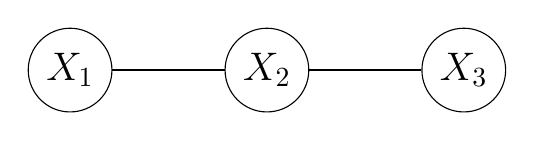
\begin{tikzpicture}[node distance=2.5cm, main node/.style={circle, draw, minimum size=1cm, font=\sffamily\Large\bfseries}]
  \node[main node] (1) {$X_1$};
  \node[main node] (2) [right of=1] {$X_2$};
  \node[main node] (3) [right of=2] {$X_3$};
  \draw[thick] (1) -- (2);
  \draw[thick] (2) -- (3);
\end{tikzpicture}
\end{center}

\subsection*{b) Valeur de la constante $\mathcal{Z}$}

La constante de normalisation $\mathcal{Z}$ s'obtient en sommant le produit des potentiels sur l'ensemble des configurations possibles pour le triplet binaire $(X_1, X_2, X_3)$ :
\[ \mathcal{Z} = \sum_{X_1, X_2, X_3 \in \{0,1\}} \phi_1(X_1, X_2) \phi_2(X_2, X_3) \]

On a alors :
\begin{itemize}
    \item $X=(1,1,1) : 10 \times 4 = 40$
    \item $X=(1,1,0) : 10 \times 3 = 30$
    \item $X=(1,0,1) : 1 \times 2 = 2$
    \item $X=(1,0,0) : 1 \times 5 = 5$
    \item $X=(0,1,1) : 1 \times 4 = 4$
    \item $X=(0,1,0) : 1 \times 3 = 3$
    \item $X=(0,0,1) : 3 \times 2 = 6$
    \item $X=(0,0,0) : 3 \times 5 = 15$
\end{itemize}

En sommant l'ensemble de ces termes, on obtient :
\[ \mathcal{Z} = 40 + 30 + 2 + 5 + 4 + 3 + 6 + 15 = 105 \]

La constante $\mathcal{Z}$ est donc égale à \textbf{105}.

\vspace{1cm}
\hrule
\vspace{1cm}

\section*{Question 6 : Réseaux bayésiens et SRM}

\subsection*{a) Expression de $\mathbb{P}(A, B, C, D, E, F)$ selon $\mathcal{G}_1$}

Selon le théorème de caractérisation des structures de réseau bayésien, la distribution jointe se factorise comme le produit des probabilités conditionnelles de chaque nœud étant donné ses parents. En observant le graphe $\mathcal{G}_1$, on déduit :
\[ \mathbb{P}(A, B, C, D, E, F) = \mathbb{P}(A)\mathbb{P}(B)\mathbb{P}(C \mid A)\mathbb{P}(D \mid A, B)\mathbb{P}(E \mid C, D)\mathbb{P}(F \mid D) \]

\subsection*{b) Construction d'une SRM (carte des indépendances minimale de $\mathbb{P}$)}

Pour construire la SRM, il faut moraliser le graphe orienté $\mathcal{G}_1$. Cela s'effectue en deux étapes :
\begin{enumerate}
    \item \textbf{Marier les parents :} On ajoute une arête non orientée entre les parents d'une même immoralité (v-structure). Ici, on relie $A$ et $B$ (parents de $D$), ainsi que $C$ et $D$ (parents de $E$).
    \item \textbf{Retirer l'orientation :} On transforme toutes les arêtes fléchées en arêtes simples non orientées.
\end{enumerate}

Le graphe $\mathcal{H}$ résultant est illustré ci-dessous (les arêtes de moralisation ajoutées sont en rouge pointillé) :

\begin{center}
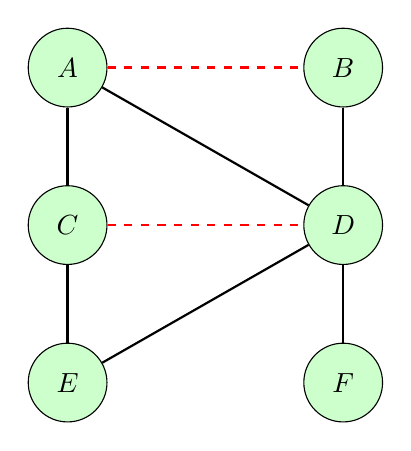
\begin{tikzpicture}[node distance=2cm, main node/.style={circle, draw, fill=green!20, minimum size=1cm, font=\sffamily\bfseries}]
  \node[main node] (A) {$A$};
  \node[main node] (B) [right of=A, xshift=1.5cm] {$B$};
  \node[main node] (C) [below of=A] {$C$};
  \node[main node] (D) [below of=B] {$D$};
  \node[main node] (E) [below of=C] {$E$};
  \node[main node] (F) [below of=D] {$F$};

  % Arêtes initiales (désorientées)
  \draw[thick] (A) -- (C);
  \draw[thick] (A) -- (D);
  \draw[thick] (B) -- (D);
  \draw[thick] (C) -- (E);
  \draw[thick] (D) -- (E);
  \draw[thick] (D) -- (F);
  
  % Arêtes de moralisation
  \draw[dashed, red, thick] (A) -- (B);
  \draw[dashed, red, thick] (C) -- (D);
\end{tikzpicture}
\end{center}

\subsection*{c) La SRM est-elle une carte parfaite des indépendances de $\mathbb{P}$ ?}

\textbf{Non.} Le processus de moralisation entraîne une perte d'informations concernant certaines indépendances. 

Par exemple, dans la distribution originale $\mathbb{P}$ (et lue par d-séparation dans $\mathcal{G}_1$), les variables $A$ et $B$ sont marginalement indépendantes ($A \indep B$). Cependant, dans la SRM construite en b), l'ajout de l'arête de moralisation crée un chemin direct et actif entre $A$ et $B$. Dans le contexte des réseaux markoviens, cela signifie qu'elles sont jugées dépendantes. 

Puisque l'ensemble des indépendances lues dans le graphe n'est plus exactement égal à celui de la distribution ($\mathcal{I}(\mathcal{H}) \neq \mathcal{I}(\mathbb{P})$), la SRM n'est pas une carte parfaite des indépendances.

\subsection*{d) Bonus : Expressions pour les fonctions de potentiel $\phi_1, \dots, \phi_4$}

On cherche à exprimer $\tilde{\mathbb{P}}(A, B, C, E, F) = \sum_{D} \mathbb{P}(A, B, C, D, E, F)$. 
Substituons l'expression trouvée en a) :
\begin{align*}
\tilde{\mathbb{P}}(A, B, C, E, F) &= \sum_{D \in \{0,1\}} \Big( \mathbb{P}(A)\mathbb{P}(B)\mathbb{P}(C \mid A)\mathbb{P}(D \mid A, B)\mathbb{P}(E \mid C, D)\mathbb{P}(F \mid D) \Big)
\end{align*}

Comme la somme ne porte que sur $D$, on peut sortir les termes indépendants de $D$ à l'extérieur de la sommation :
\[ \tilde{\mathbb{P}}(A, B, C, E, F) = \mathbb{P}(A)\mathbb{P}(B)\mathbb{P}(C \mid A) \sum_{D \in \{0,1\}} \Big( \mathbb{P}(D \mid A, B)\mathbb{P}(E \mid C, D)\mathbb{P}(F \mid D) \Big) \]

En identifiant cette forme avec le produit demandé $\phi_1(A)\phi_2(B)\phi_3(A, C)\phi_4(A, B, C, E, F)$, on obtient des expressions tout à fait cohérentes :
\begin{itemize}
    \item $\phi_1(A) = \mathbb{P}(A)$
    \item $\phi_2(B) = \mathbb{P}(B)$
    \item $\phi_3(A, C) = \mathbb{P}(C \mid A)$
    \item $\phi_4(A, B, C, E, F) = \displaystyle \sum_{D \in \{0,1\}} \mathbb{P}(D \mid A, B)\mathbb{P}(E \mid C, D)\mathbb{P}(F \mid D)$
\end{itemize}
\

\section*{Question 7}

\subsection*{a) SRB}

\begin{figure}[H]
    \centering
    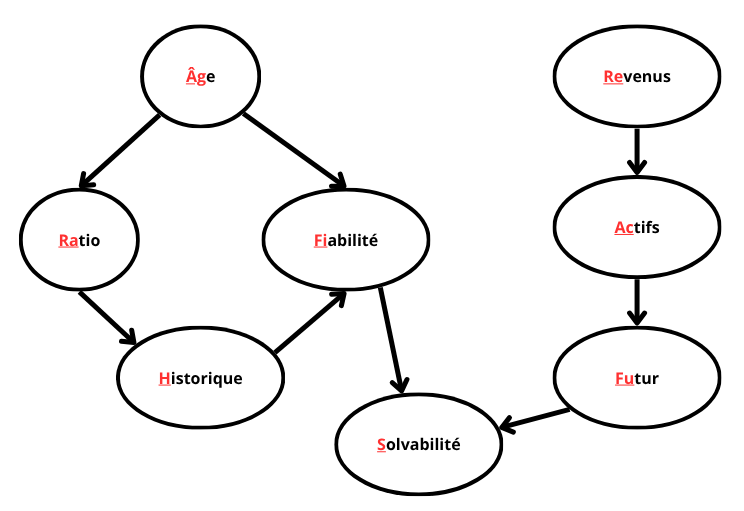
\includegraphics[width=1\linewidth]{Q7.png}
    \caption{SRB de la situation décrite par Claude}
\end{figure}

L'hypothèse de Claude est validée par les énoncés rapportés : la solvabilité des clients dépend de leur fiabilité et de leur revenus futurs.

\subsection*{b) Distribution jointe}

Par simplicité, on désigne chaque variable par sa section soulignée en rouge dans la figure ci-dessus. \\
La distribution jointe s'exprime alors :

\begin{align*}
\mathbb{P}(&\text{Ag, Ra, Fi, H, Re, Ac, Fu, S}) \\ 
&= \mathbb{P}(\text{Ag})  \cdot \mathbb{P}(\text{Re}) \\
&\quad \cdot \mathbb{P}(\text{Ra} \mid \text{Ag}) \cdot \mathbb{P}(\text{Ac} \mid \text{Re}) \\
&\quad \cdot \mathbb{P}(\text{H} \mid \text{Ra}) \cdot \mathbb{P}(\text{Fu} \mid \text{Ac}) \\
&\quad \cdot \mathbb{P}(\text{Fi} \mid \text{Ag, H}) \cdot \mathbb{P}(\text{S} \mid \text{Fi, Fu})
\end{align*}

\subsection*{c) Table de probabilités conditionnelles : P(Ratio | Âge)}

L'éenoncé 3 indique : "Plus un(e) client(e) est âgé(e), plus il/elle a tendance à avoir un faible ratio dettes vs revenus;"

\

Voici alors un exemple de valeurs cohérentes avec l'énoncé :

\begin{table}[H]
    \centering
    \renewcommand{\arraystretch}{1.3}
    \begin{tabular}{|l|c|c|c|c|} \hline
        \textbf{Âge} & \textbf{$\mathbb{P}(\text{Ratio} = \text{Élevé})$} & \textbf{$\mathbb{P}(\text{Ratio} = \text{Moyen})$} & \textbf{$\mathbb{P}(\text{Ratio} = \text{Faible})$} & \textbf{Total} \\ \hline
        Moins de 25 ans & 0.67 & 0.21 & 0.12 & 1.0 \\ \hline
        Entre 25 et 50 & 0.42 & 0.32 & 0.26 & 1.0 \\ \hline
        Entre 50 et 65 & 0.21 & 0.35 & 0.44 & 1.0 \\ \hline
        65 et plus & 0.05 & 0.21 & 0.74 & 1.0 \\ \hline
    \end{tabular}
\end{table}

Ces valeurs arbitraires respectent l'hypothèse car on observe bien que la probabilité d'obtenir un ratio de dettes "Faible" augmente plus la personne est âgée.

\end{document}
